\subsection{香美市の高齢者の割合}
高知県産業振興推進部統計分析課によると、令和5年の香美市の年齢別人口および割合は次のようになっている。

\begin{figure}[h]
  \centering
  \begin{minipage}{0.43\columnwidth}
    \centering
    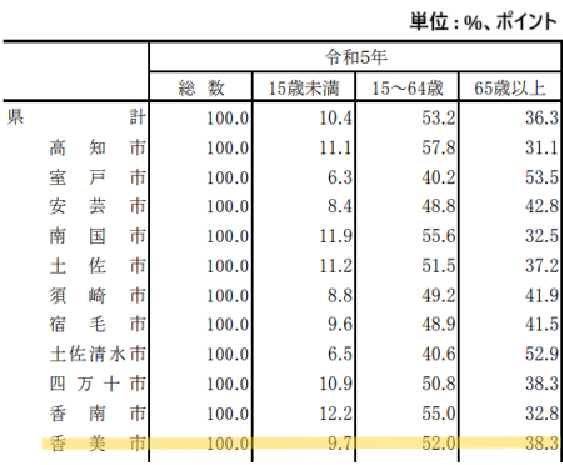
\includegraphics[width=\columnwidth]{population_rate.pdf}
    \caption{市町村別の年齢別人口}
    \label{fig:サンプルA}
  \end{minipage}
  \hspace{5mm}
  \begin{minipage}{0.43\columnwidth}
    \centering
    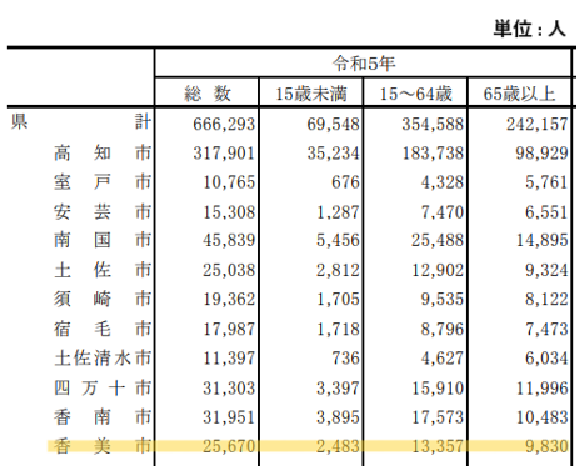
\includegraphics[width=\columnwidth]{population.pdf}
    \caption{市町村別の年齢別人口割合}
    \label{fig:サンプルB}
  \end{minipage}
\end{figure}

%年齢別人口(上位5位)のグラフをここに追加するかどうか?

この統計から、香美市の総人口は25,670人であり、そのうち高齢者(高齢者)は約9,800人で全体の4割近くを占めていることが分かる。また、香美市は高知県内の市町村の中でも65歳以上の人口が第5位に位置しており、県内でも特に高齢者人口が多いことが分かる。

今後も人口減少や少子高齢化の進行によって、高齢者の割合がさらに増加する可能性が高い。そのため、働き手となる世代が減少する一方で、生活支援を必要とする高齢者が増えるという問題と向き合っていかなければならない。

このような背景から、香美市では高齢者の生活を支える新たな仕組みづくりや、地域住民が安心して暮らせる環境整備が必要であると考えられる。特に、買い物や移動といった日常生活のサポート体制をどう確保するかが今後の重要な課題である。



\subsection{生活用品を確保する手段}
中山間地域を中心とした概ね50世帯未満の集落を対象に実施された「令和3年度高知県集落実態調査」によると、食料品などの生活必需品を確保する際に困難や課題を感じている人が全体の6割以上にのぼることが明らかになっている。
特に中山間地域では、「移動手段がない」「移動販売の頻度が少ない」といった問題が多く挙げられており、買い物環境の不便さが日常生活に大きな影響を及ぼしていることが分かる。
さらに、令和2年国勢調査を基にした集落調査データによれば、香美市では50世帯未満の小規模集落が全体の65.9\%を占めている。
このことから、香美市内においても同様に、移動手段の不足や移動販売の機会の少なさが深刻な課題となっていると考えられる。


\begin{figure}[h]
  \centering
  \begin{minipage}{0.43\columnwidth}
    \centering
    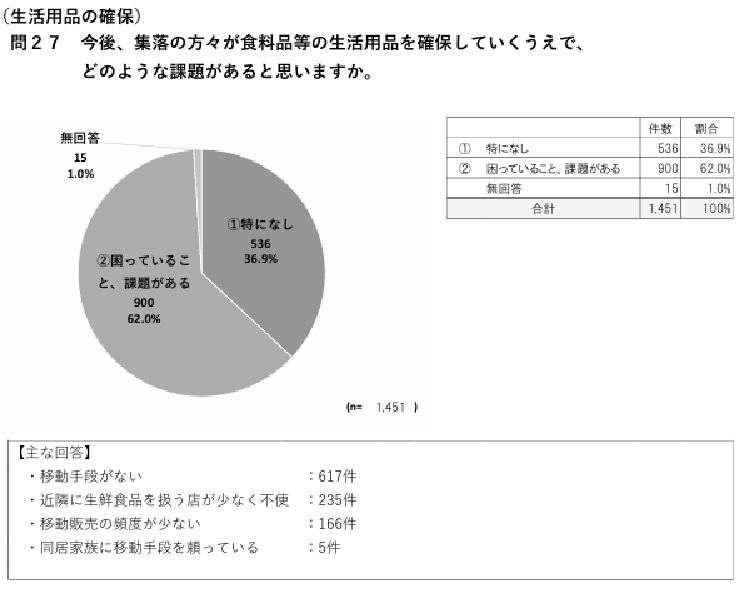
\includegraphics[width=\columnwidth]{get_food_graph.pdf}
    \caption{生活用品確保のための課題}
    \label{fig:get_food}
  \end{minipage}
  \hspace{5mm}
  \begin{minipage}{0.43\columnwidth}
    \centering
    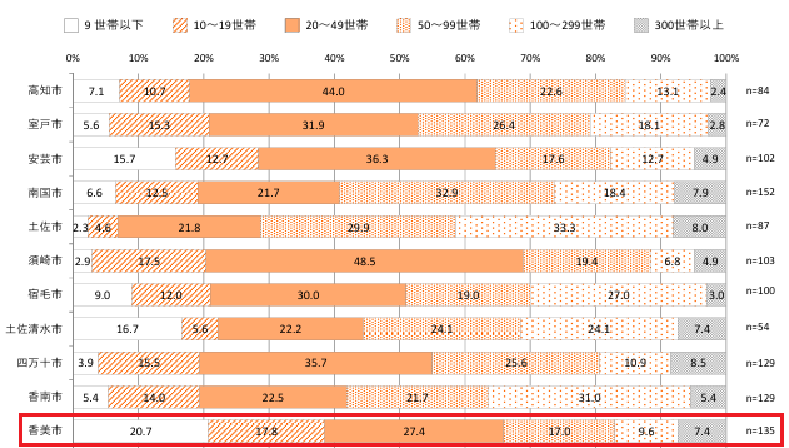
\includegraphics[width=\columnwidth]{市町村別世帯数別集落数の割合.pdf}
    \caption{香美市の世帯数別集落数の割合}
    \label{fig:市町村別世帯数別集落数の割合}
  \end{minipage}
\end{figure}

\subsection{移動手段の確保}

図 \ref{fig:免許}は、高知県における人口と運転免許証保有者数を示したものである。令和3年時点での免許保有者数は約45.5万人にのぼり、年齢別に見ると「45~49歳」が最も多く、次いで「70~74歳」の保有者が多いことが分かる。さらに、75歳以上の後期高齢者でも約4.7万人が免許を保有していることから、多くの高齢者が日常生活において自家用車を移動手段として利用している現状がうかがえる。
しかし、加齢に伴う身体機能の低下や認知機能の変化により、今後は運転の継続が困難となる高齢者が増加すると考えられる。その結果、自動車以外の移動手段を持たない高齢者が外出や買い物を行うことが難しくなり、生活用品の確保に苦労する人がさらに増える可能性が高い。


\begin{figure}[H]
  \centering
  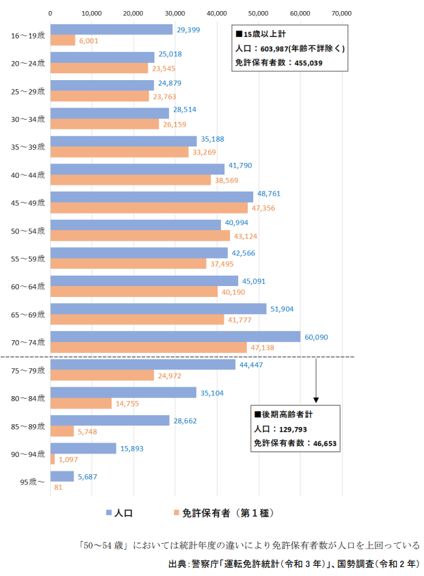
\includegraphics[width=0.5\textwidth]{免許証.png}
  \caption{高知県の人口と免許証保有者数}
  \label{fig:免許}
\end{figure}


\subsection{学生のバイト先の不足}
高知工科大学の学生102名にアンケート調査を行ったところ、図 \ref{fig:アンケート} のような結果が得られた。 
この結果から、全体の79.4\%の学生が香美市内で働くことを希望しているにも関わらず、実際に「香美市内にアルバイト先が十分にある」と感じている学生は12.8\%にとどまっていることが分かる。 
つまり、働く意欲を持つ学生に対して、香美市内ではそれを受け入れるだけの雇用機会が十分にはないという深刻な現状が明らかになっている。 
香美市は高知工科大学を有し、多くの学生が生活している地域であるにも関わらず、応募できる職種や店舗が限られており、「働きたいのに働けない」状況が常態化していると考えられる。 

\begin{figure}[h]
  \centering
  \begin{minipage}{0.43\columnwidth}
    \centering
    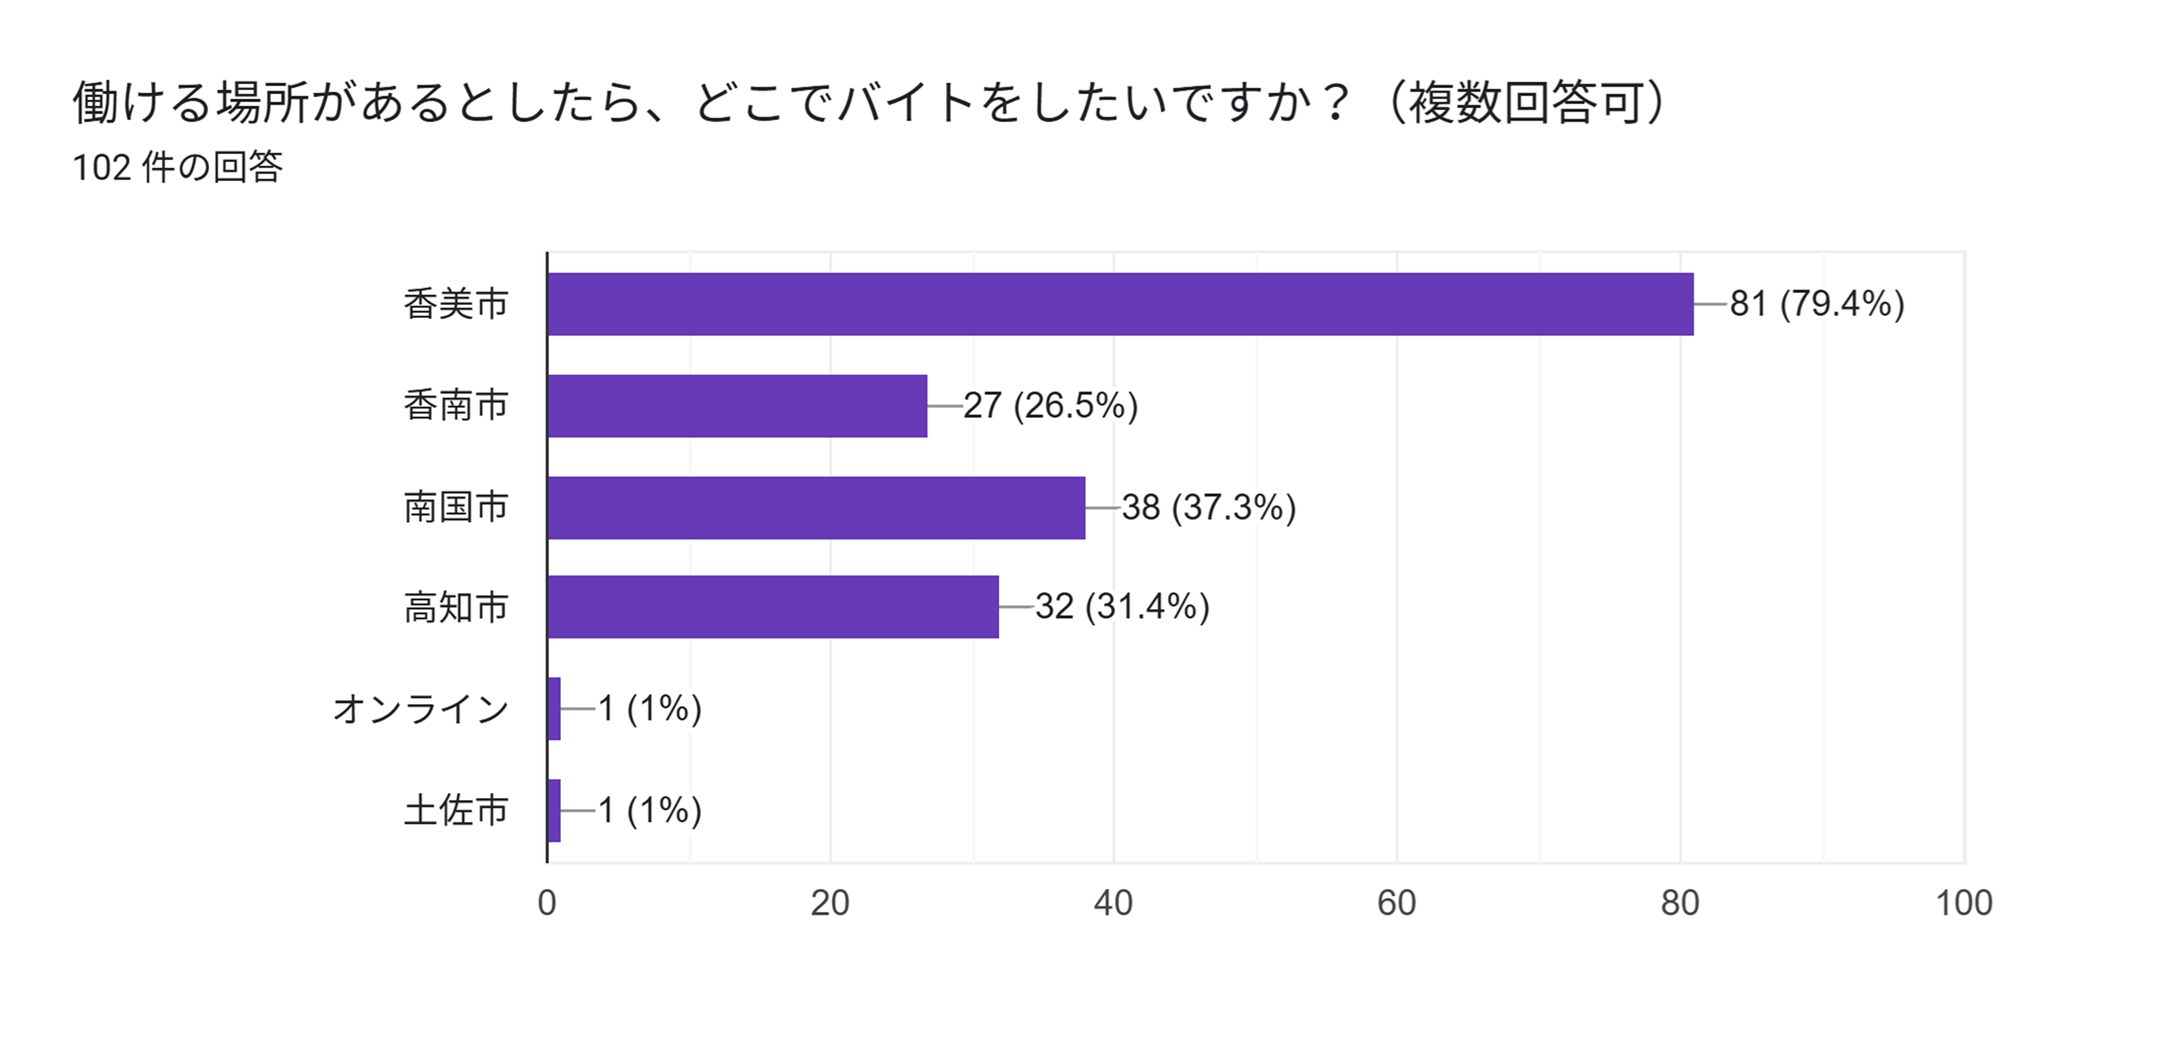
\includegraphics[width=\columnwidth]{働く場所の希望_アンケート結果.png}
  \end{minipage}
  \hspace{5mm}
  \begin{minipage}{0.43\columnwidth}
    \centering
    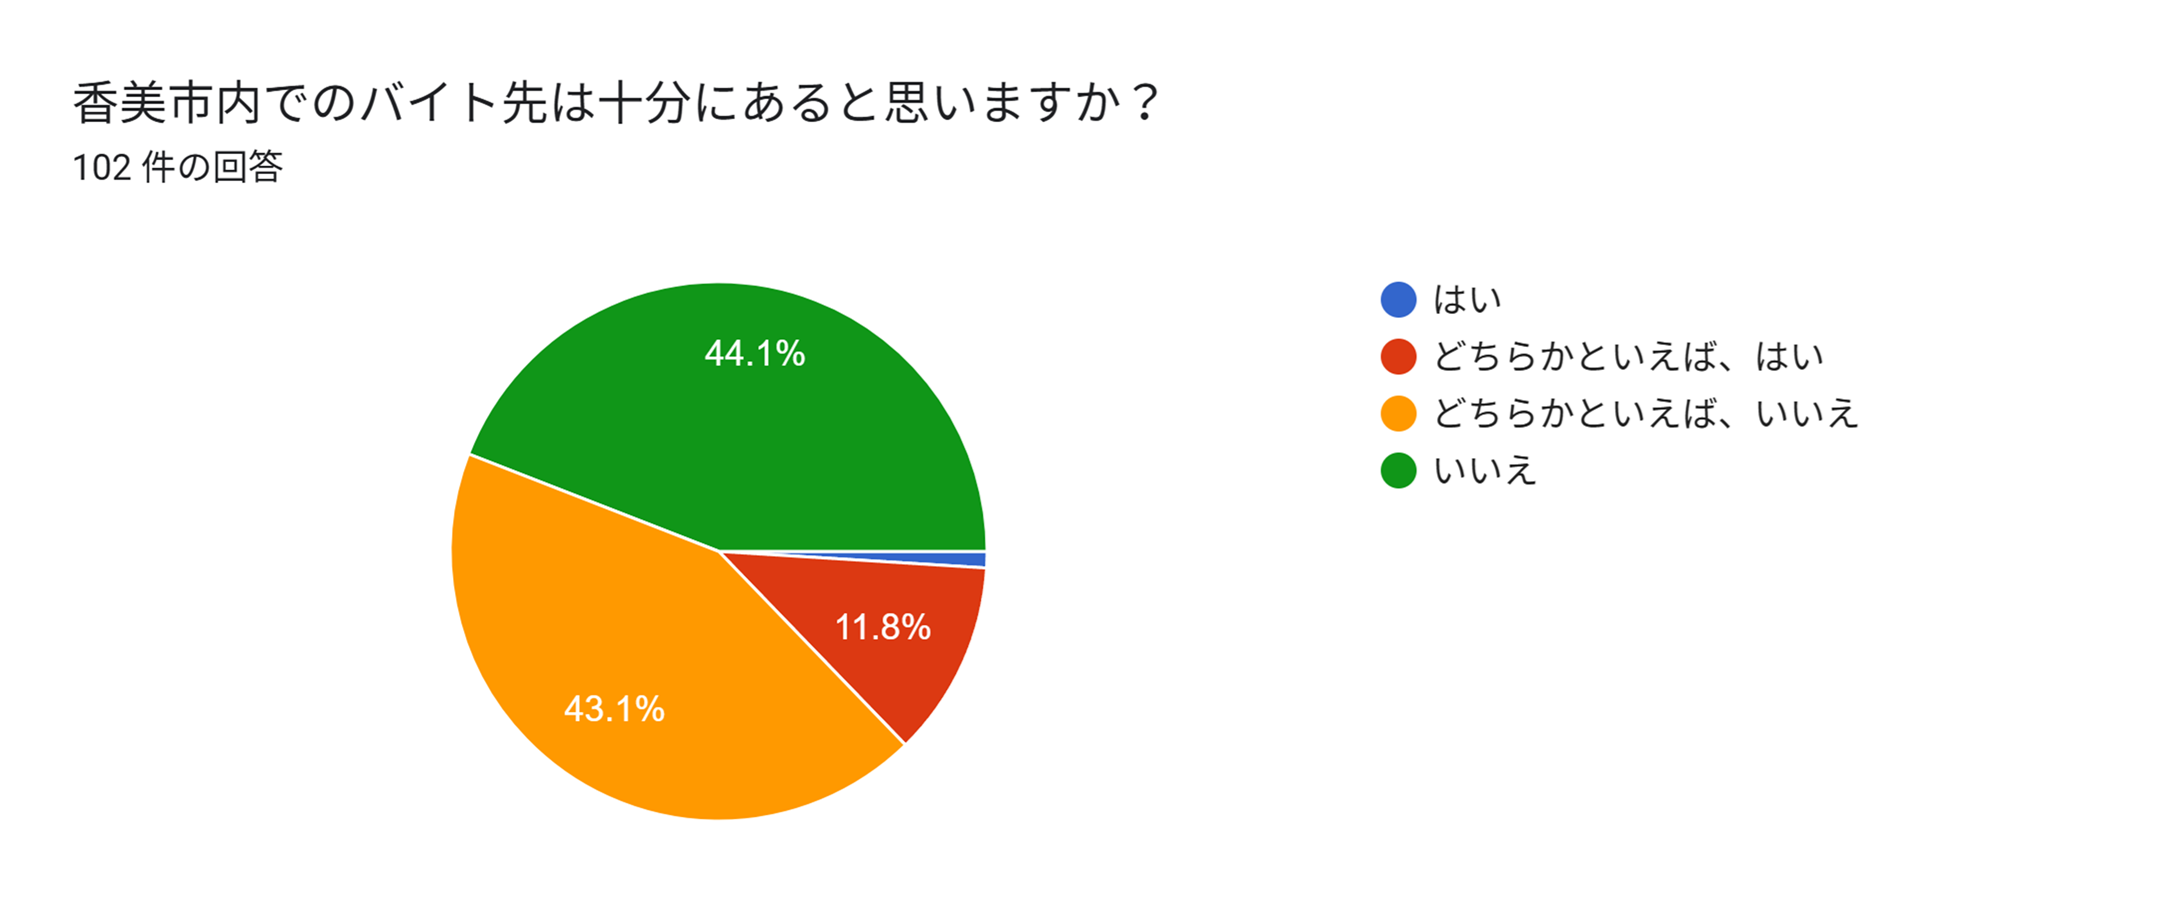
\includegraphics[width=\columnwidth]{香美市でのバイト先が十分にあるか_アンケート結果.png}
  \end{minipage}
  \caption{バイト先に関するアンケート調査結果}
  \label{fig:アンケート}
\end{figure}
%未完成
